\subsection{Far-field scattering} \label{sec:ff_scattering}


\begin{figure}[h] %  figure placement: here, top, bottom, or page
   \centering
   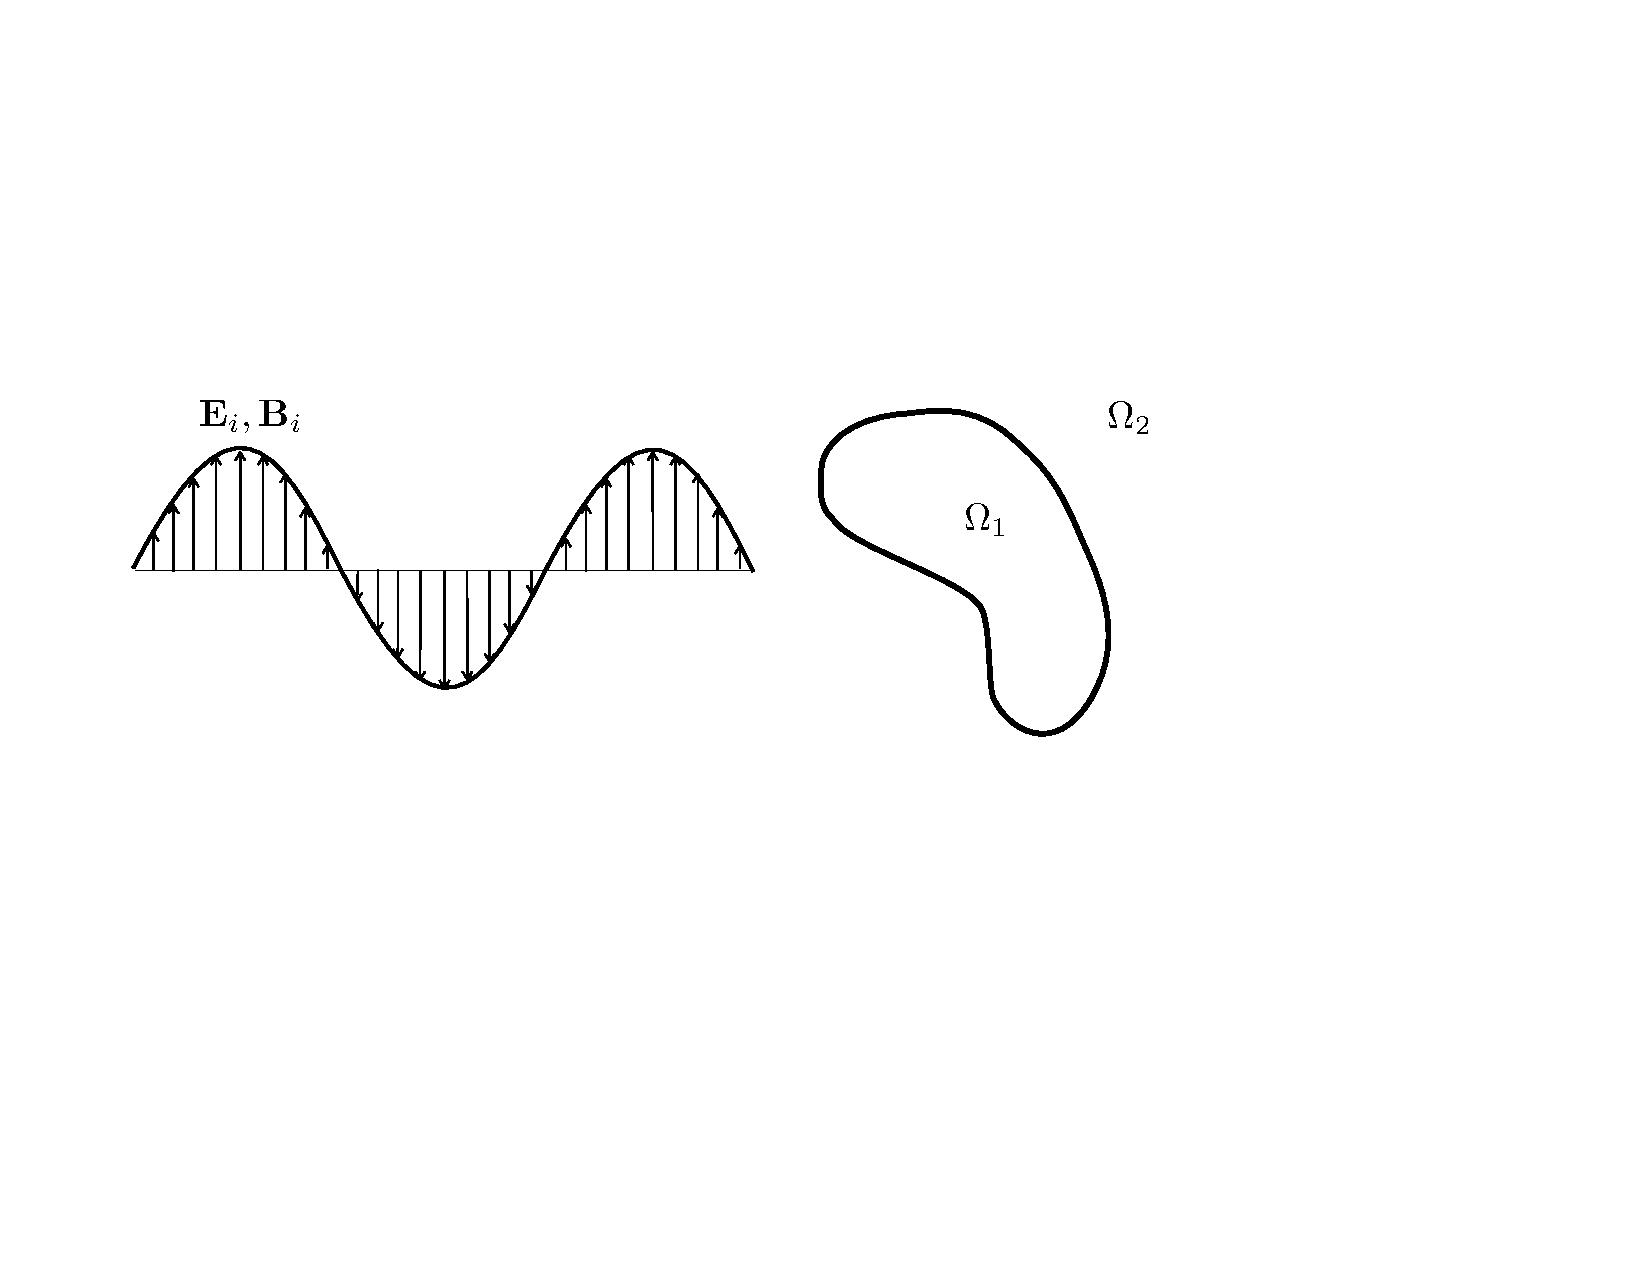
\includegraphics[width=0.45\textwidth]{particle_wave.pdf} 
   \caption{Nanoparticle under electromagnetic wave.}
   \label{fig:part_wave}
\end{figure}

In LSPR computations, we measure the scattered electromagnetic field on a detector
that is located far away from the nanoparticle. When light shines on an object 
like in Figure \ref{fig:part_wave}, the incident wave ($\mathbf{E}_i$,  $\mathbf{B}_i$)
is scattered along the domain, resulting in a total electromagnetic field 
($\mathbf{E}$,  $\mathbf{B}$) that depends on the incoming wave, the particle's 
geometry, and the material constants. In the quasistatic approximation, we only
 need to compute the electric field and the magnetic contribution can be 
neglected \cite{MayergoyzZhang2007}. In the far-field limit, the scattered field
in the outside region ($\Omega_2$) is given by: 

\begin{equation} \label{eq:scat_efield_long_range}
    \mathbf{E}_{2s} = \frac{1}{4\pi\epsilon_2}k^2\frac{e^{ikr}}{r} (\mathbf{\hat{r}} \times \mathbf{p})\times\mathbf{\hat{r}}.
\end{equation} 

\noindent where $k=2\pi/\lambda$ is the wave number and $\lambda$ the wavelength, $\mathbf{\hat{r}}$ 
is a unit vector in the direction of the observation point, and $\mathbf{p}$ is
the dipole moment.

We can also obtain the scattered field with the forward-scattering amplitude 
\cite{Jackson}:

\begin{equation} \label{eq:scat_efield_fwa}
    \mathbf{E}_{2s}(\mathbf{r})_{r\to\infty} = \frac{e^{ikr}}{r} \mathbf{F}(\mathbf{k},\mathbf{k}_0),
\end{equation}

\noindent where $\mathbf{F}$ is the forward-scattering amplitude, $\mathbf{k}$ is the 
scattered wave vector in the direction of propagation, and $\mathbf{k}_0$ the 
wave vector of the incident field. 

Via these two equations, we use \pygbe to compute the scattered electric field 
and then solve for the forward-scattering amplitude. 

\subsection{Extinction cross-section and Optical theorem} \label{sec:cext_ot}

The extinction cross-section quatifies how much extinction (scattered + absorbed) 
is caused by a particle when this one is shinned with light. It is defined as the
ratio between the extinct energy and the intensity of the incoming wave. 

The optical theorem relates the extinction cross-section with the forward-scattering amplitude. The traditional expression for this relationship applies for non-absorbing media \cite{MayergoyzZhang2007, Jackson}. The expression for absorbing media \cite{BohrenGilra1979, VideenSun2003} was corrected by Mishchenko \cite{Mishchenko2007}, giving the following expression:

\begin{equation} \label{eq:cext_fwa}
    C_\text{ext} = \frac{4\pi}{k^\prime} \operatorname{Im} \left[ \frac{\mathbf{\hat{e}}_i}{|\mathbf{E}_i|}\mathbf{F}(\mathbf{k}=\mathbf{k}_0, \mathbf{k}_0) \right].
\end{equation}


{\color{red}{Chris in Mishenko 2007 paper the equation is not exactly the same 
(look eq 87 in paper), do you have that derivation? How you got to the eq 7.22 
 in your thesis?.}}


Here, $k^\prime$ is the real part of the complex wave number. 

\begin{equation}
    k = k^\prime + ik^{\prime\prime} = \frac{2\pi}{\lambda} n,
\end{equation}

and $n$ is the refraction index of the host medium.


\subsection{Boundary integral formulation} \label{sec:lspr_bem}

\subsubsection{Electrostatic potential under an incoming electric field}

From the electrostatic approximation from Mayergoyz and Zhang (2007) 
\cite{MayergoyzZhang2007} we know that the zeroth order term of the magnetic 
field is zero everywhere. Resulting in the following Maxwell equations. 

\begin{align} \label{eq:electrostatic_scatter_E}
\nabla \cdot \mathbf{E}^{(0)}_{1s} &= 0 \qquad \nabla \times \mathbf{E}^{(0)}_{1s} = 0 \nonumber \\
\nabla \cdot \mathbf{E}^{(0)}_{2s} &= 0 \qquad \nabla \times \mathbf{E}^{(0)}_{2s} = 0 \nonumber \\
(\epsilon_1\mathbf{E}^{(0)}_{1s} - \epsilon_2\mathbf{E}^{(0)}_{2s})\cdot\mathbf{n} &= (\epsilon_2-\epsilon_1)\mathbf{E}_i\cdot \mathbf{n}.
\end{align}

Where the subscript $s$ ($i$) stands for scattered (incident) field. The curl of
$\mathbf{E}^{(0)}_{js}$ for $j=1,2$ is zero, therefore, there is a scalar potential
such that $-\nabla \phi_js = \mathbf{E}^{(0)}_js$. Using this, we can rewrite 
equation \eqref{eq:electrostatic_scatter_E} as:

\begin{align} \label{eq:electrostatic_scatter}
\nabla^2 \phi_{1s} &= 0 \qquad \nabla^2 \phi_{2s} = 0 \qquad\text{on $\Omega_1$, $\Omega_2$} \nonumber \\
\epsilon_1\frac{\partial\phi_{1s}}{\partial \mathbf{n}} - \epsilon_2\frac{\partial\phi_{2s}}{\partial\mathbf{n}} &= (\epsilon_2-\epsilon_1)\frac{\partial\phi_i}{\partial\mathbf{n}} \quad \phi_{1s} = \phi_{2s} \quad \text{on $\Gamma$}.
\end{align}

\paragraph{Week formulation and layer operators}


The weak formulation of Laplace equation with test function $w$:

\begin{equation} \label{eq:lap_weak}
\int_\Omega \nabla^2 \phi(\mathbf{r}_\Omega') w(\mathbf{r}_\Omega') \text{d} \Omega^\prime= 0.
\end{equation}

\noindent where the evaluation point is $\mathbf{r}_\Omega$ a location in the domain $\Omega$.

If we use the Laplace's free-space Green's function as the test function $w$ we
get:

\begin{equation} \label{eq:lap_weak2}
\int_\Omega \nabla^2 \phi(\mathbf{r}'_\Omega) G_L(\mathbf{r}_\Omega,\mathbf{r}'_\Omega) \text{d} \Omega^\prime= 0.
\end{equation}

Manipulating the integrand using the product rule and later the divergence 
theorem, we get:

\begin{equation} \label{eq:lap_bie_dom}
\phi(\mathbf{r}_\Omega) = \int_\Gamma G_L(\mathbf{r}_\Omega,\mathbf{r}'_\Gamma)  \frac{\partial} {\partial \mathbf{n}} \phi(\mathbf{r}'_\Gamma)  \text{d} \Gamma^\prime - \int_\Gamma \phi(\mathbf{r}'_\Gamma)  \frac{\partial}{\partial \mathbf{n}} G_L(\mathbf{r}_\Omega,\mathbf{r}'_\Gamma) \text{d} \Gamma^\prime
\end{equation}

\noindent where \eqref{eq:lap_bie_dom}, $\mathbf{r}$ can be anywhere in the domain $\Omega$, 
and $\mathbf{r}'$ runs only on the boundary $\Gamma$. This equation has a 
singularity when $\mathbf{r}=\mathbf{r}'$. To handle thisproblem, we perform the
integral on a surface $\Gamma'$ that is like $\Gamma$ but with a hemisphere of 
radius $\varepsilon$ center at $\mathbf{r}$. We split the integrals into the part
that we have no singularity and the part that has the hemisphere. After solving these
equations when $\varepsilon \to 0$, equation \eqref{eq:lap_bie_dom} results in:

\begin{equation} \label{eq:lap_bie}
\frac{\phi(\mathbf{r}_\Gamma)}{2} +  \int_\Gamma \phi(\mathbf{r}'_\Gamma)  \frac{\partial}{\partial \mathbf{n}} G_L(\mathbf{r}_\Gamma,\mathbf{r}'_\Gamma) \text{d} \Gamma^\prime = \int_\Gamma G_L(\mathbf{r}_\Gamma,\mathbf{r}'_\Gamma)  \frac{\partial} {\partial \mathbf{n}} \phi(\mathbf{r}'_\Gamma)  \text{d} \Gamma^\prime,
\end{equation}

\noindent where these are Cauchy principal value integrals.

Using the single and double layer operators:

{\color{red} Chris, V is single layer operator but is it K the double layer one? 
In your thesis you have that the double layer is W and you refers as K as
"an operator" eq 2.108 and 2.112 in your thesis. Also shouldn't the $\text{d} \Gamma$
be $\text{d} \Gamma'$? }

\begin{equation}\label{eq:single_layer}
V^{\mathbf{r}_\Gamma}_L (\psi(\mathbf{r}_\Gamma)) = \int_\Gamma \psi(\mathbf{r}'_\Gamma) G_L(\mathbf{r}_\Gamma, \mathbf{r}'_\Gamma) \text{d} \Gamma.
\end{equation}

\begin{equation}\label{eq:double_layer}
K^{\mathbf{r}_\Gamma}_L (\psi(\mathbf{r}_\Gamma)) = \int_\Gamma \psi(\mathbf{r}'_\Gamma) \frac{\partial}{\partial \mathbf{n}}G_L(\mathbf{r}_\Gamma, \mathbf{r}'_\Gamma) \text{d} \Gamma.
\end{equation}

We can rewrite equation \eqref{eq:lap_bie} using the operator notation, as:

\begin{equation} \label{eq:lap_operator}
\left[ \frac{\mathbb{I}}{2} + K_L^{\mathbf{r}_\Gamma} \right] \left( \phi_\Gamma \right) = V_L^{\mathbf{r}_\Gamma} \left( \frac{\partial}{\partial \mathbf{n}} \phi_\Gamma \right),
\end{equation}

\noindent where $\mathbb{I}$ is the identity operator.

Following the same stepps, we can rewrite the Laplace equations in eqaution
\eqref{eq:electrostatic_scatter} as:

%
\begin{align} \label{eq:integral_eq_lspr_nobc}
\frac{\phi_{1s,\Gamma}}{2}+ K_{L}^{\Gamma}(\phi_{1s,\Gamma}) - V_{L}^{\Gamma} \left(\frac{\partial}{\partial \mathbf{n}}\phi_{1s,\Gamma} \right) = 0&  \nonumber \\
\frac{\phi_{2s,\Gamma}}{2} - K_{L}^{\Gamma}(\phi_{2s,\Gamma}) + V_{L}^{\Gamma} \left( \frac{\partial}{\partial \mathbf{n}} \phi_{2s,\Gamma} \right) = 0& \quad \text{on $\Gamma$,}
\end{align}

Applying the interface conditions of Equation \eqref{eq:electrostatic_scatter},
we get:

\begin{align} \label{eq:integral_eq_lspr}
\frac{\phi_{1s,\Gamma}}{2}+ K_{L}^{\Gamma}(\phi_{1s,\Gamma}) - V_{L}^{\Gamma} \left(\frac{\partial}{\partial \mathbf{n}}\phi_{1s,\Gamma} \right) = 0&  \nonumber \\
\frac{\phi_{1s,\Gamma}}{2} - K_{L}^{\Gamma}(\phi_{1s,\Gamma}) + \frac{1}{\epsilon_2}V_{L}^{\Gamma} \left( \epsilon_1 \frac{\partial}{\partial \mathbf{n}} \phi_{1s,\Gamma} - (\epsilon_2-\epsilon_1) \frac{\partial}{\partial \mathbf{n}} \phi_{i,\Gamma} \right) = 0& \quad \text{on $\Gamma$.}
\end{align}


\paragraph{Discretization and Linear system}


We discretize the surface into flat triangles, and assume that  $\phi$ and 
$\partial \phi/\partial \mathbf{n}$ are constant within each panel. Then, we can
write the layer operators in their discretized form:

\begin{align} \label{eq:layers_disc}
V_{L,\text{disc}}^{\mathbf{r}_i} \left( \frac{\partial}{\partial \mathbf{n}} \phi(\mathbf{r}_{\Gamma}) \right) &= \sum_{j=1}^{N_p} \frac{\partial}{\partial \mathbf{n}} \phi(\mathbf{r}_{\Gamma_j}) \int_{\Gamma_j} G_L(\mathbf{r}_{i},\mathbf{r}_{\Gamma_j})  \mathrm{d} \Gamma_j  \nonumber \\
K_{L,\text{disc}}^{\mathbf{r}_i}(\phi(\mathbf{r}_{\Gamma})) &=  \sum_{j=1}^{N_p}\phi(\mathbf{r}_{\Gamma_j})\int_{\Gamma_j} \frac{\partial}{\partial \mathbf{n}} \left[ G_L(\mathbf{r}_{i},\mathbf{r}_{\Gamma_j}) \right]\mathrm{d} \Gamma_j
\end{align}

\noindent where $N_p$ is the number of discretization elements of $\Gamma$, 
and $\phi(\mathbf{r}_{\Gamma_j})$ and $\frac{\partial}{\partial \mathbf{n}} 
\phi(\mathbf{r}_{\Gamma_j})$ are the values of $\phi$ and 
$\frac{\partial \phi}{\partial \mathbf{n}}$ on panel $\Gamma_j$.


Then we can write equation \eqref{eq:integral_eq_lspr} in matrix form as:
%
 \begin{equation} \label{eq:matrix_lspr}
 \left[
    \begin{matrix} 
       \frac{1}{2} + K_{L}^{\Gamma} & -V_{L}^{\Gamma}  \vspace{0.2cm} \\
       \frac{1}{2} - K_{L}^{\Gamma} &  \frac{\epsilon_1}{\epsilon_2} V_{L}^{\Gamma}  \vspace{0.2cm} 
    \end{matrix}
    \right] \left[ 
    \begin{matrix} 
       \phi_{1s,\Gamma} \vspace{0.2cm} \\
       \frac{\partial}{\partial \mathbf{n}} \phi_{1s,\Gamma} \vspace{0.2cm}
    \end{matrix} 
     \right] =   
    \left[
    \begin{matrix} 
       0 \\
       V_{L}^{\Gamma} \left(\frac{\epsilon_2-\epsilon_1}{\epsilon_2}\right) \frac{\partial\phi_i}{\partial\mathbf{n}} \vspace{0.2cm} 
    \end{matrix}
    \right]
 \end{equation}

\noindent where the elements of the matrices are
%
\begin{align} \label{eq:layers_element}
V_{L,ij}^{\Gamma} &= \int_{\Gamma_j} G_L(\mathbf{r}_{\Gamma_i},\mathbf{r}_{\Gamma_j})  \mathrm{d} \Gamma_j \nonumber \\
K_{L,ij}^{\Gamma} &= \int_{\Gamma_j} \frac{\partial}{\partial \mathbf{n}} \left[ G_L(\mathbf{r}_{\Gamma_i},\mathbf{r}_{\Gamma_j}) \right]\mathrm{d} \Gamma_j
\end{align}

\noindent with $\mathbf{r}_{\Gamma_i}$ at the center of $\Gamma_i$.

\paragraph{Integral evaluation}

To evaluate the integrals in Equation \eqref{eq:layers_element} we use quadrature
rules. However, the Green's function of the Laplace equation has a $1/r$
singularity, which is a problem to obtain good accuracy when the integral is 
singular or near-singular. Therefore, we define three different regions:

\emph{Far-away integrals:} The collocation point and the integration panel are 
dar away. We can obtain good accuracy with a low order integration, for example 
$K=1, 3 \; or \; 4$ Gauss quadrature points per boundary element. To define a 
threshold from which collocation points are considered to be far away, we use a
representative length of the integrated triangle, $L = \sqrt{2\cdot\text{Area}}$.

\emph{Near-singular integrals:} The collocation point is closer than the far-away
region threshold, but it's not in the same integration panel, we use high order 
Gauss quadrature rules $K_{fine}=19, 25 \; or \; 37$ points per triangle. 

\emph{Singular integrals:} Having the collocation point in the integrated panel
introduces a singularity that keeps us from computing theintegral with standard
Gauss integration schemes. In this case, we use a semi-analytical technique from
Zhe and co-workers \cite{ZhuHuangSongWhite2001} which gives us an accurate
integration of the Laplace potential.
{\color{red}Chris I can't find an explanation on how is it that the Nk parameter
applies here. I know it is "number of Gauss points per triangle edge for
semi-analytical integration" but where is that explained? can you add that part?}

\subsubsection{Boundary integral expression of the dipole moment}

As shown in Equation \eqref{eq:scat_efield_long_range}, the scattered electric 
field in the far-away limit depends on the dipole moment. The dipole moment is 
defined as 

%
\begin{equation} \label{eq:dipole_def}
\mathbf{p} = \int_\Omega \mathbf{r} \rho \text{d}\Omega,
\end{equation}

Rewriting this equation using Gauss's law we obtain
%
\begin{equation} \label{eq:dipole_def_gauss}
\mathbf{p} = -\epsilon_2\int_\Omega \mathbf{r} \nabla^2 \phi_{2s} \text{d}\Omega.
\end{equation}


{\color{red} Here is where we need to sort out the sign problem in equations and 
how we write the derivation. Will fix when we talk with Chris}


\subsection{Acceleration startegies} \label{sec:acc_strategies}

One downside of the Boundary Elements Method (\bem) is that the resulting matrix obtained
after discretization, is dense. Solving the linear system using the traditional 
Gaussian elimination requires $\O{N^3}$ computations and $\O{N^2}$ storage. Using
an iterative solver, like the Generalized Minimal Residual Method (\gmres),
scaling drops to $\O{N^2}$ since computations are dominated by the matrix-vector 
product. This makes \bem a good approach for only few thousands boundary elements,
which is far from the mesh sizes required for real applications. Fortunately, there
are acceleration methods, like Barnes and Hut Treecode \cite{BarnesHut1986} that
make the computations scale as $\O{N \log N}$, that allows us to use \bem for 
larger problems. 

The Barnes-Hut Treecode is a fast-summation algorithm capable of reducing $\O{N^2}$
computational patterns 

\begin{equation} \label{eq:summation}
V(\mathbf{x}_i) = \sum_{j=1}^{N} q_j \psi(\mathbf{x}_i, \mathbf{y}_j) 
\end{equation}

\noindent to a computational complexity of $\O{N \log N}$. Where $q_j$ is the 
weight, $\psi$ the kernel, $\mathbf{y}_j$ the location of sources and 
$\mathbf{x}_i$ the location of targets.

\pygbe uses the treecode to accelerate the \bem solver by aggregating the
far-away sources to a center of expansion that interacts with the target location. 
In the treecode, we group the sources $\mathbf{y}_j$ depending on their positions
in cells or boxes of an octree. Then, we compute the nearby contributions directly,
and approximate the further contributions using series expansions representing
the sources around the box centers  $\mathbf{y}_c$. In this work we use Taylor 
series for the expansions of order $P$ (parameter picked depending on the siumlation).
To decide if a box of sources is distant enough of each target point for the Taylor
expansion approximation, we use the multiple-acceptance criterion $\theta$ (MAC). This
must be larger than the ratio of the box's size to the distance between the target
and box's center $\frac{r_b}{r}<\theta$. Common values for $\theta$ are
$\frac{1}{2}$ and $\frac{2}{3}$.  

You can find further detail on the Treecode implementation in \pygbe in Cooper, 
et al (2013) \cite{CooperBardhanBarba2013}. 













